\chapter{Experimental Setup}

\section{Training}

\subsection{Model Training Configuration}

The optimal hyperparameter configuration identified through our experimental campaign is detailed in \cref{tab:hyperparameters}. Subsequent analyses and results are reported based on the parameters optimized during this primary training run.

A critical architectural modification was the introduction of a task gain hyperparameter, $z_\mathrm{gain}$. Preliminary experiments revealed a failure mode where the predictive model marginalized the task latent $\mathbf{z}$, instead over-relying on the temporal continuity of the visual latent sequence $\mathbf{e}_t$. Given the high sampling frequency of the dataset, the predictor could achieve a deceptively low loss by effectively performing an identity mapping of the current state. By scaling the task latent by $z_\mathrm{gain}$, we force the optimization process to treat the semantic task specification as a primary causal factor in state transitions.

Training stability was further ensured through the implementation of gradient norm clipping and weight decay. The CLIP-based text encoder parameters ($\phi$) were fine-tuned via Parameter-Efficient Fine-Tuning (PEFT) rather than being held frozen, allowing the linguistic features to align with the specific visual manifold of the robotic environment. To maintain architectural consistency, CLIP embeddings were projected from their native 512-dimensional space to the 192-dimensional latent space of the \texttt{ViT-Tiny} encoder using a learnable linear projection $W_\phi : \mathbb{R}^{d_z} \to \mathbb{R}^d$. Computational operations were executed on an NVIDIA RTX A4500 GPU equipped with \qty{20}{\giga\byte} of VRAM.

\begin{table}[htbp]
	\centering
	\caption{Model architecture and training hyperparameters.}
	\label{tab:hyperparameters}
	\begin{tabular}{llc}
		\toprule
		\textbf{Category} & \textbf{Hyperparameter}                   & \textbf{Value} \\
		\midrule
		\multirow{5}{*}{Architecture}
		                  & Embedding Dimension ($d$)                 & 192            \\
		                  & Task Latent Dimension ($d_z$)             & 512            \\
		                  & Attention Heads                           & 4              \\
		                  & Transformer Layers                        & 12             \\
		                  & Task Gain Factor ($z_{\text{gain}}$)      & 10.0           \\
		\midrule
		\multirow{8}{*}{Training}
		                  & Batch Size                                & 256            \\
		                  & Buffer Size                               & 2048           \\
		                  & Learning Rate (Encoder)                   & $\num{1e-4}$   \\
		                  & Learning Rate (Predictor)                 & $\num{1e-4}$   \\
		                  & Learning Rate (Goal Encoder)              & $\num{3e-4}$   \\
		                  & Weight Decay                              & 0.05           \\
		                  & Training Epochs                           & 3              \\
		                  & Gradient Clipping Norm                    & 1.0            \\
		\midrule
		\multirow{4}{*}{Loss Weights}
		                  & Predictive Loss ($\lambda_{\text{pred}}$) & 1.0            \\
		                  & SIGReg Loss ($\lambda_{\text{SIGReg}}$)   & 0.02           \\
		                  & Rollout Loss ($\lambda_{\text{RO}}$)      & 0.002          \\
		                  & Rollout Steps ($K$)                       & 16             \\
		\midrule
		\multirow{3}{*}{LoRA}
		                  & Rank ($r$)                                & 8              \\
		                  & Alpha ($\alpha$)                          & 16             \\
		                  & Dropout                                   & 0.1            \\
		\bottomrule
	\end{tabular}
\end{table}

\nomenclature{$z_{\text{gain}}$}{Scaling factor for the task latent to prevent task-marginalization}
\nomenclature{$W_\phi$}{Learnable linear projection for task-vision latent alignment}

\subsection{Dataset Specification}

The latent predictive EBM was trained on a custom dataset comprising \num{12000} robot manipulation episodes. The environment consists of a tabletop workspace featuring three multi-colored primitives (cubes) interacting with a robotic manipulator. Visual observations $o_t$ are RGB images resized to $224 \times 224$ pixels. Each episode is paired with a semantic task description $\tau \in \Sigma^\ast$, such as $\tau = \text{``Lift the red cube''}$, which defines the goal-conditioned behavior for that trajectory. \cref{fig:dataset} illustrates representative samples of visual observations and their associated linguistic instructions.

\begin{figure}[htbp]
	\begin{center}
		\begin{subfigure}{0.45\textwidth}
			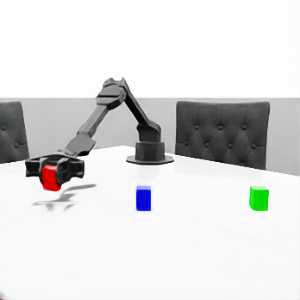
\includegraphics[width=\textwidth]{figures/dataset/pick-red.png}
			\caption{``Lift the red cube''}
		\end{subfigure}
		\hfill
		\begin{subfigure}{0.45\textwidth}
			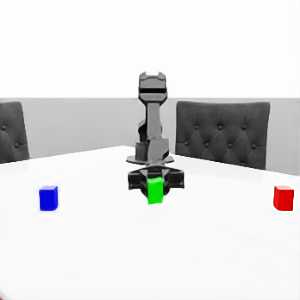
\includegraphics[width=\textwidth]{figures/dataset/pick-green.png}
			\caption{``Lift the green cube''}
		\end{subfigure}
	\end{center}
	\caption{\textbf{Dataset Samples.}\ Visual observations captured during the terminal phase of successful manipulation episodes.}
	\label{fig:dataset}
\end{figure}

\section{Generative Qualitative Visualization}

To ground the model's internal representations in the visual domain, we train a convolutional decoder $D_\gamma: \mathbb{R}^d \to \mathcal{I}$ specifically to map latent vectors back to the image manifold. This allows for the visualization of ``imagined'' rollout sequences generated by the autoregressive mechanism. Given an initial state $o_0$ and a ground-truth task $\tau$, we also introduce a counterfactual task $\tau' \neq \tau$ to assess the model's task-discriminative reasoning. We generate two distinct $K$-step latent trajectories:
\begin{subequations}
	\begin{align}
		\mathbf{e}_0            & = g_\theta(o_0)                                                                          \\
		\hat{\mathbf{e}}_{1:K}  & = \mathsc{Rollout}(\mathbf{e}_0, g_\phi(\tau), h_\theta, K) \label{eq:open_ro_correct}   \\
		\hat{\mathbf{e}}'_{1:K} & = \mathsc{Rollout}(\mathbf{e}_0, g_\phi(\tau'), h_\theta, K) \label{eq:open_ro_wrong}    \\
		\hat{o}_{1:K}           & = D_\gamma(\hat{\mathbf{e}}_{1:K})                           \label{eq:decoding_correct} \\
		\hat{o}'_{1:K}          & = D_\gamma(\hat{\mathbf{e}}'_{1:K}) \label{eq:decoding_wrong}
	\end{align}
\end{subequations}
The resulting image sequences, $\hat{o}_{1:K}$ and $\hat{o}'_{1:K}$, provide a qualitative window into the model’s predictive capabilities. Furthermore, we evaluate the decoder's reconstruction fidelity by mapping ground-truth latents back to the image space:
\begin{equation}
	\tilde{o}_{0:K} = D_\gamma(g_\theta(o_{0:K})) .
	\label{eq:reconst_obs}
\end{equation}

\nomenclature{$D_\gamma$}{Convolutional decoder for latent-to-image reconstruction}
\nomenclature{$\gamma$}{Parameters of the convolutional decoder}
\nomenclature{$\tilde{o}$}{Reconstructed visual observation}

\section{Task-Conditioning Performance}

A robust goal-conditioned model must demonstrate high sensitivity to the provided task specification $\tau$. We quantify this sensitivity by measuring the L2-norm between the predicted latent sequence and the ground-truth latent sequence under two conditions: the correct task $\tau$ and a counterfactual (wrong) task $\tau'$. At each timestep $t$, we compute the following error metrics:
\begin{subequations}
	\begin{align}
		E_t  & = \| \hat{\mathbf{e}}_{t} - \mathbf{e}_{t} \|^2_2 \label{eq:err_ro_correct}  \\
		E'_t & = \| \hat{\mathbf{e}}'_{t} - \mathbf{e}_{t} \|^2_2 , \label{eq:err_ro_wrong}
	\end{align}
\end{subequations}
where $\hat{\mathbf{e}}_{t}$ and $\hat{\mathbf{e}}'_{t}$ represent the predicted states for the correct and counterfactual tasks, respectively. To characterize the discriminative power of the model throughout the training process, we define the Task Sensitivity Index
\begin{equation}
	\beta = \mathbb{E}\left[\frac{E'_t}{E_t}\right] .
	\label{eq:task_sens}
\end{equation}
An increasing $\beta$ indicates that the model is successfully learning to differentiate between semantic instructions and is producing task-appropriate future predictions.

\nomenclature{$\beta$}{Task Sensitivity Index; ratio of counterfactual to concordant prediction error}
\nomenclature{$E_t, E'_t$}{Prediction error at time $t$ for correct and counterfactual tasks, respectively}

\section{Latent Manifold Analysis}

The structure of the latent manifold learned by $g_\theta$ is characterized through dimensionality reduction, specifically via Principal Component Analysis (PCA). We project the predicted trajectories from \cref{eq:open_ro_correct} and \cref{eq:open_ro_wrong} along with the ground-truth latent trajectory $\mathbf{e}_{0:K}$ into the primary principal components. This visualization allows us to inspect the ``reasoning'' paths the model takes in the latent space.

Finally, to empirically validate the effectiveness of SIGReg in mitigating latent collapse, we perform a comparative visualization. We contrast the latent distribution of an encoder trained with SIGReg against a baseline model trained without regularization, illustrating how SIGReg maintains the information-theoretic spread of the latent space.

\nomenclature{PCA}{Principal Component Analysis}
\nomenclature{VRAM}{Video Random Access Memory}
\nomenclature{GPU}{Graphics Processing Unit}

